In this chapter we will go through different methods we used to verify the multigrid
solver, as well as scaling measurements. Modular parts of the solver is tested with unittests
where feasible. In addition the whole solver is tested with both analytically solvable
test cases and randomly generated fields.


\subsection{Error Quantification}
	\label{sec:errorQuant}
	In order to evaluate solutions we will primarily look at the normalized 2-norm of the error, \cref{eq:2norm},
	and the residual, \cref{eq:barRes}. The \(\norm{ err }_2\) is computed from comparing the numerical
	solution \(\hat{\phi}\) to an analytical solution \(\phi\) and normalized with regards to grid points, \(N\).
	The residual is found by inserting the numerical solution into the Poisson equation, the remaining
	part is then the residual, and shows the difference of the current numerical solution
	and the optimal numerical solution.
	%
	\begin{align}
		\norm{ err }_2&= \sqrt{\frac{\sum \left(\hat\phi - \phi\right)^2}{N}}  \label{eq:2norm}
		\\
		\bar{r} &= \frac{1}{N}\left( \sum_i{ \nabla^2 \hat{\phi}_i + \rho_i  }  \right) \label{eq:barRes}
	\end{align}
	%
	% \subsection{Analytical Solutions}
	% 	We use a few different constructed charge density fields, which is analytically solvable,
	% 	to test the performance and correctness of the solver. All the simulations here are ran on
	% 	a grid of the size \( 128, 64, 64 \) divided into \(1,2,2\) subdomains.
 % 		It uses \(5\) cycles when presmoothing, solving on the coarsest grid and postsmoothing, the
	% 	MG solver is instructed to run for \(100\) MG V-cycles with \(2\) grid levels.
	%
	% \subsubsection{Sinusoidal function}
	% 	\label{sec:sinusoidal}
	% 	A sinusoidal source term, \(\rho\) can be useful to test the solver since
	% 	it can be constructed to have very simple derivatives and integrals. Here
	% 	we use a sinusoidal function that has two positive tops and two negative tops
	% 	over the total domain. We want the sinus function to go over \(1\) period
	% 	over the domain, so we normalize the argument by dividing the grid point
	% 	value, \(x_j, y_k, z_l\), by the domain length in the direction, \(L_x, L_y, L_z\).
	%
	% 	\begin{align}
	% 		\rho(x_j,y_j,z_l) &= \sin\left( x_j \frac{2\pi}{L_x} \right)\sin\left( y_{k} \frac{2\pi}{L_y} \right)
	% 		\intertext{A potential that fits with this is:}
	% 		\phi(x,y,z) &= -\left(\frac{2\pi}{L_x}\right)^2\left(\frac{2\pi}{L_y}\right)^2
 % 			\sin\left( x_j \frac{2\pi}{L_x} \right)\sin\left( y_{k} \frac{2\pi}{L_y} \right)
	% 	\end{align}
	%
	% 	\begin{figure}
	% 		\centering
	% 			% \begin{subfigure}[b]{0.32\textwidth}
	% 			% 	\includegraphics[width = \textwidth]{figures/verification/sinusoidal/rho.pdf}
	% 			% \end{subfigure}
	% 			% \begin{subfigure}[b]{0.32\textwidth}
	% 			% 	\includegraphics[width = \textwidth]{figures/verification/sinusoidal/phi.pdf}
	% 			% \end{subfigure}
	% 			% \begin{subfigure}[b]{0.32\textwidth}
	% 			% 	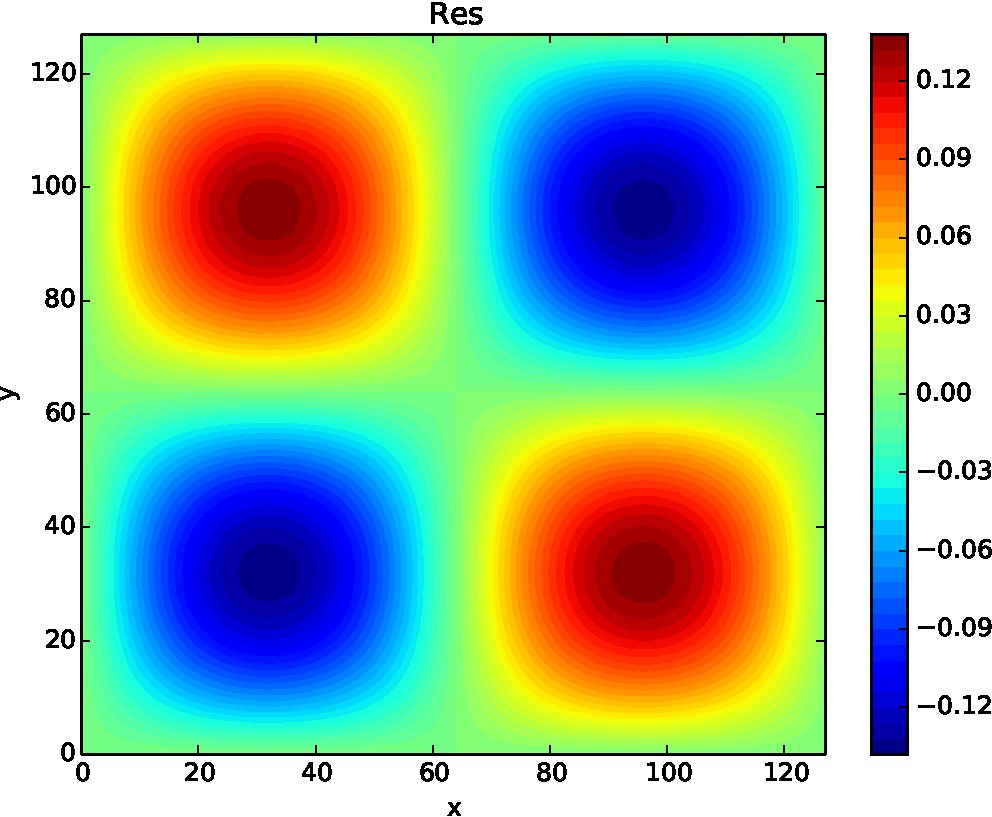
\includegraphics[width = \textwidth]{figures/verification/sinusoidal/residual.pdf}
	% 			% \end{subfigure}
	% 		\caption{This a \(x,y\)-plane from the grids cut along \(z_l = 32\), from the sinusoidal test case described in \cref{sec:sinusoidal}.
	% 		The left plot shows the charge distribution, the center plot shows the numerical solution of the potential and the plot to the right depicts
	% 		the residual.}
	% 		\label{fig:sinusoidal}
	% 	\end{figure}
	%
	% 	The \cref{fig:sinusoidal} shows the results from running the MG-solver on the test sinusoidal test case described here.
	% 	As can be expected the potential mirrors the charge distribution, except with an opposite sign and a larger amplitude.
	% 	A decently large grid was simulated and the mean residual was found to be: \(\bar{r} \approx 0.0312\).
	%
	%
	% 	\subsubsection{Heaviside Function}
	% 		The solver is also tested with a charge distribution governed by a Heaviside
	% 		function. This is also suited to testing since the charge distribution is then
	% 		constant planes, and we expect second order polynomial when integrating them.
	% 		In the test case there are two planes with the value \(-1\) and two
	% 		planes with \(1\). In \cref{fig:heaviside} the test case, as well as the solution and residual is
	% 		shown, and we can see the polynomials in the solution. The mean residual \(\bar{r}\) was
	% 		\(0.00677\).
	%
	% 	\begin{align}
	% 		\rho_(x_j,y_k,z_l) &= \begin{cases} 1  & y_j \epsilon (0, 32), (64,96)\\ -1  & y_j \epsilon (33, 65), (97,127) \end{cases}
	% 	\end{align}
	%
	% 	\begin{figure}
	% 		\centering
	% 			% \begin{subfigure}[b]{0.32\textwidth}
	% 			% 	\includegraphics[width = \textwidth]{figures/verification/heaviside/rho.pdf}
	% 			% \end{subfigure}
	% 			% \begin{subfigure}[b]{0.32\textwidth}
	% 			% 	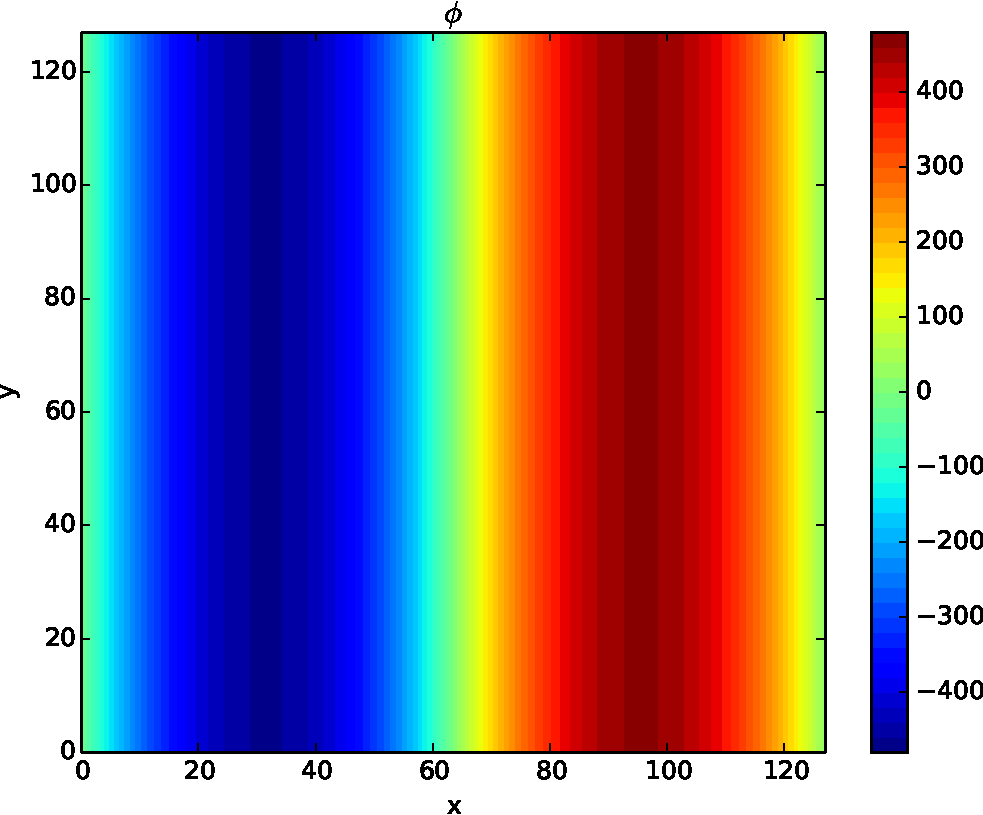
\includegraphics[width = \textwidth]{figures/verification/heaviside/phi.pdf}
	% 			% \end{subfigure}
	% 			% \begin{subfigure}[b]{0.32\textwidth}
	% 			% 	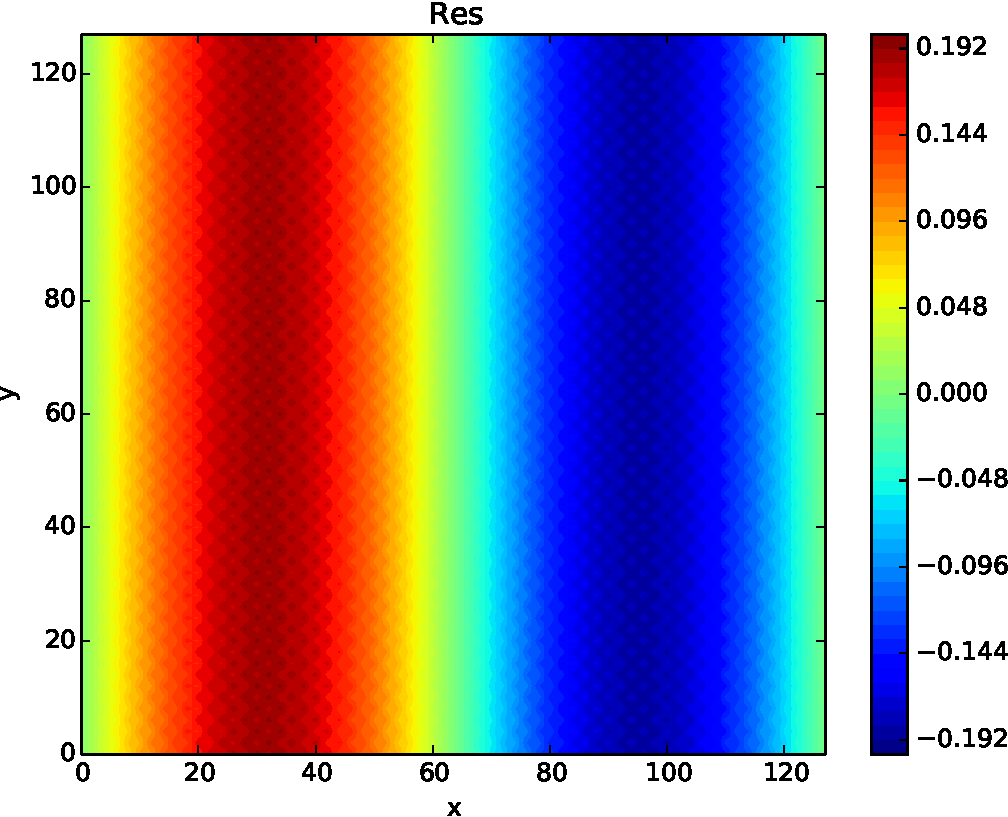
\includegraphics[width = \textwidth]{figures/verification/heaviside/residual.pdf}
	% 			% \end{subfigure}
	% 		\caption{As earlier this is a \(x,y\)-plane cut along \(x_k=32\), of the grid. The plots show the charge distribution,
	% 		numerical solution and the solution, from left to right. This is a test case constructed
	% 		with Heaviside functions. In the solution of the potential the expected second degree polynomial can be seen.
	% 		}
	% 		\label{fig:heaviside}
	% 	\end{figure}
	%
	% 	\subsection{Random Charge distribution}
	% 		To hopefully avoid some problems, that could appear due to the earlier test
	% 		cases being to constructed being to orderly, a test with a randomized
	% 		charge distribution is also included. The \cref{fig:random} shows the
	% 		charge distribution, numerical potential and the residual. The mean residual was
 % 			found to be \(\bar{r} \approx 0.00388\).
	% 		%
	% 		\begin{figure}
	% 			\centering
	% 			% \begin{subfigure}[b]{0.32\textwidth}
	% 			% 	\includegraphics[width = \textwidth]{figures/verification/random/rho.pdf}
	% 			% \end{subfigure}
	% 			% \begin{subfigure}[b]{0.32\textwidth}
	% 			% 	\includegraphics[width = \textwidth]{figures/verification/random/phi.pdf}
	% 			% \end{subfigure}
	% 			% \begin{subfigure}[b]{0.32\textwidth}
	% 			% 	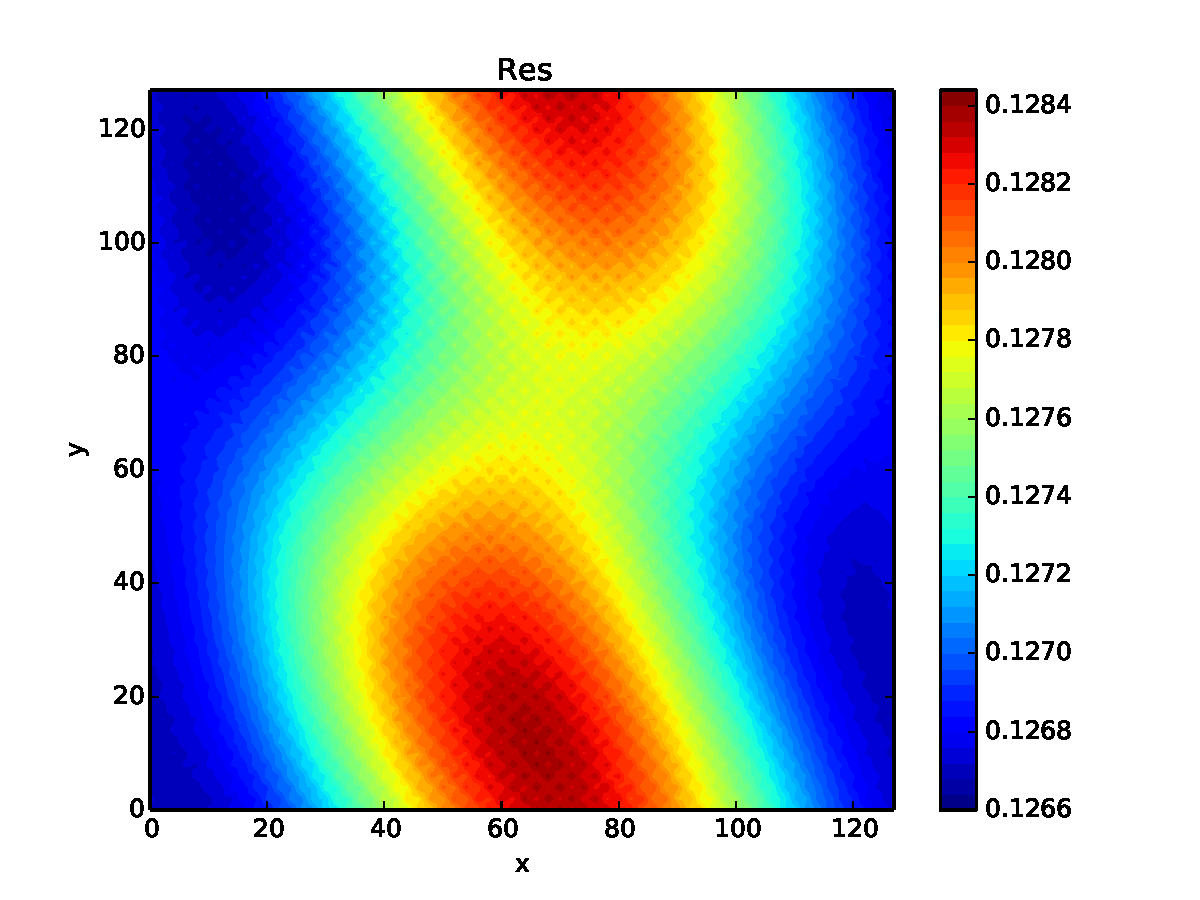
\includegraphics[width = \textwidth]{figures/verification/random/residual.pdf}
	% 			% \end{subfigure}
	% 			\caption{As earlier this is a \(x,y\)-plane cut along \(x_k=32\), of the grid. The plots show the charge distribution,
	% 			numerical solution and the solution, from left to right.}
	% 			\label{fig:random}
	% 		\end{figure}
%
% \section{Multigrid Solver}
% 	To test the solver itself we employ a couple different techniques. First we
% 	create a charge distribution by differentiating a known potential, and then
% 	running the solver and check if the resulting potential was equal to the original
% 	known potential.
%
% 	For the second test we use a charge distribution with a known analytical solution,
% 	and we then check that the solver reproduces the known analytical solution.
%
% 	A third method we use to verify it is to produce a random charge potential
% 	and then check that the potential converges, or in other words
% 	that the residual goes toward zero.
%
% 	Then lastly we use the solver on identical charge distributions with the domain
% 	divided up into different subdomains and check that the solver produces the same
% 	potential.
% \subsection{Predetermined Potential}
% 		In this section we first decide which potential we want, then numerically
% 		construct a corresponding charge potential by derivating. Then we compare the
% 		result with the original potential.

		% In
		%
		% \begin{figure}
		% 	\centering
		% 		\begin{subfigure}
		% 	% 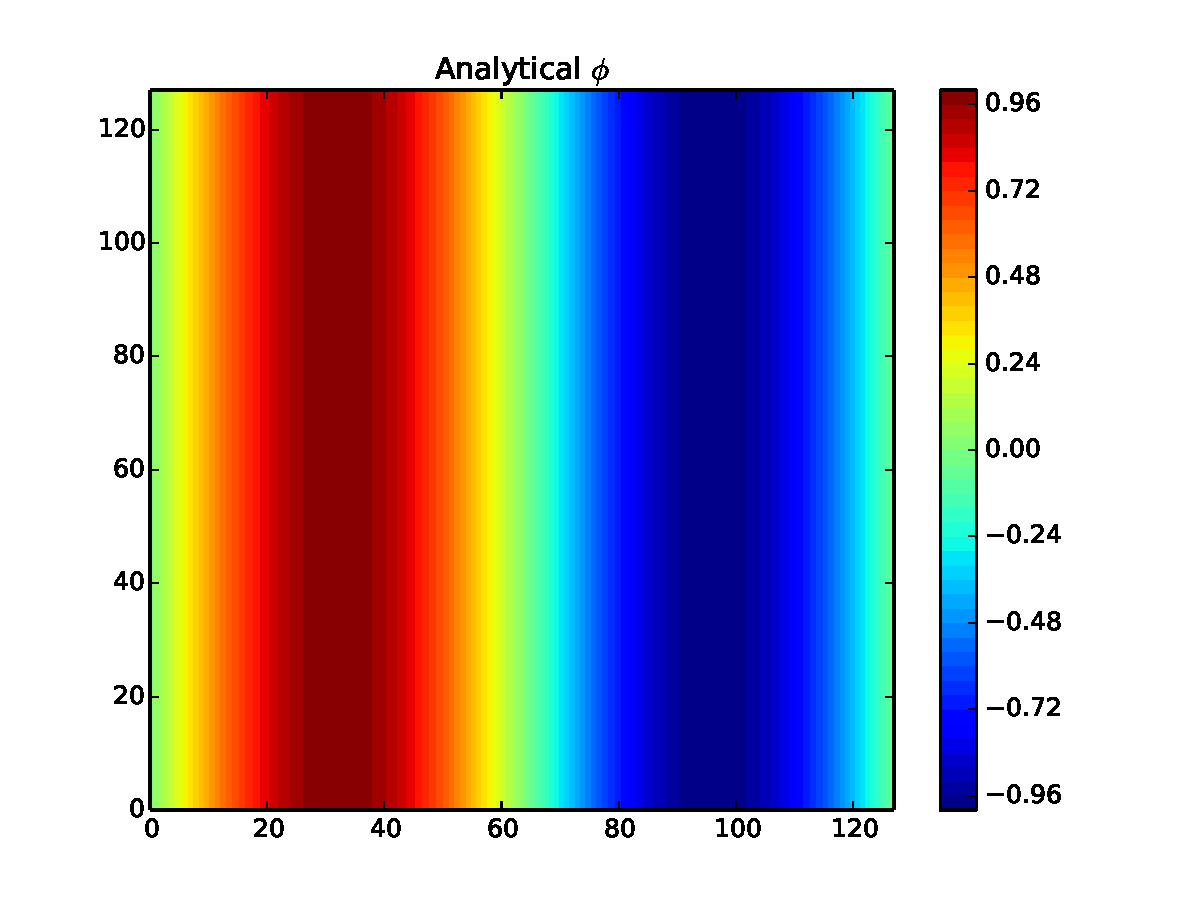
\includegraphics[width = 0.45\textwidth]{figures/verification/sinusoidal/analytical.pdf}
		% 	\end{subfigure}
		% 		\begin{subfigure}
		% 	% 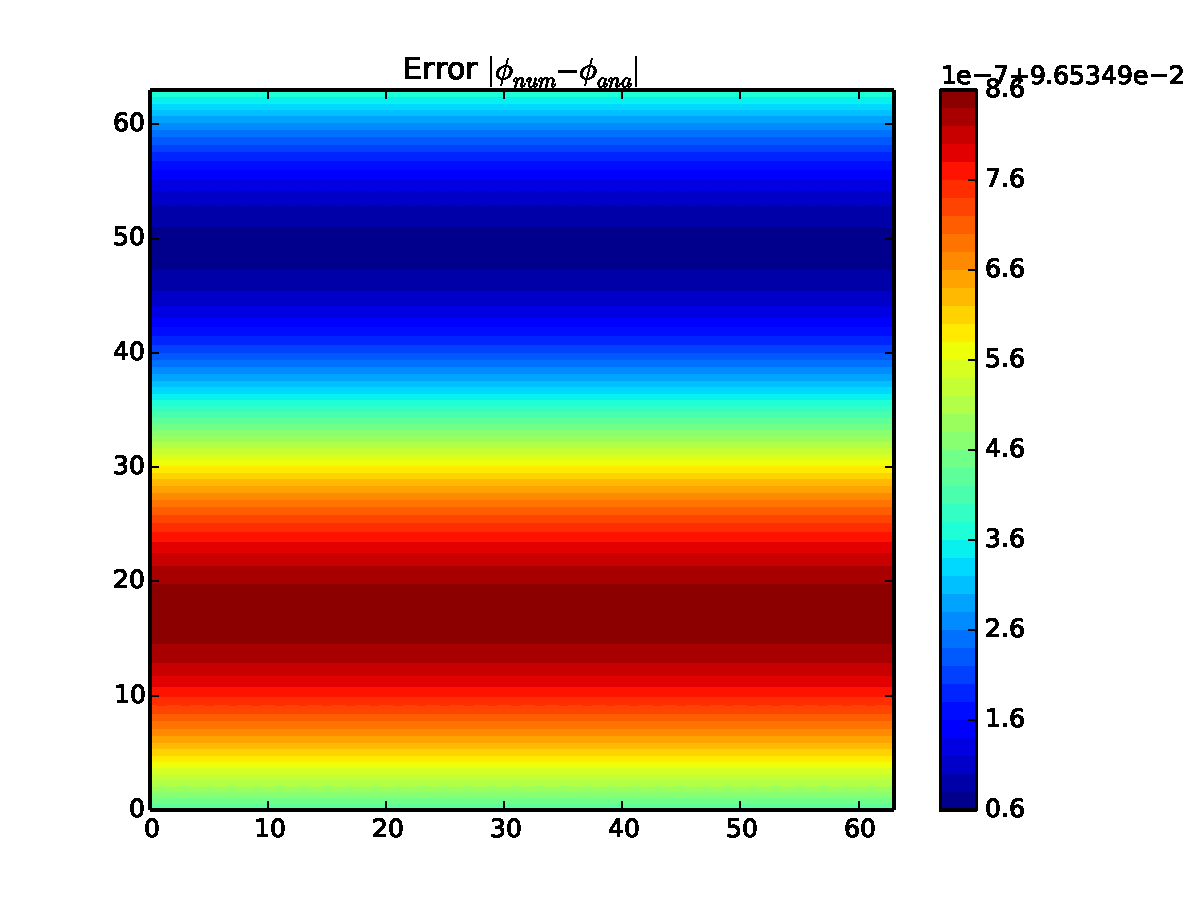
\includegraphics[width = 0.45\textwidth]{figures/verification/sinusoidal/error.pdf}
		% \end{subfigure}
		% \end{figure}
		%



		\subsection{Convergence of Residual}

		\subsection{Different Domain divisions}

% \section{Particle-in-Cell}
%
% 	\subsection{Plasma Oscillations}
%
% \textbf{NB! See if something below is salvageable}
%
%
% The multigrid method has several different steps in the algorithm, as a developmental
% help and to ensure that the program works correctly during as many different conditions
% as possible we want to test the whole code, as well as the constituent parts where possible.
% The method is quite modular and several parts of it can be tested alone.
% The GS-RB, used for smoothing, can be independently tested, since on it's own it converges to a solution,
% just at a higher computational cost than the multigrid method. To test it we will
% use an initial density field with a length between the grid steps that results in
% an exact answer. The restriction and prolongation operators can also tested to a
% degree by checking that they preserve a constant grid through several grid level changes.
%
%
% The multigrid method has several different steps in the algorithm, as a developmental
% help and to ensure that the program works correctly during as many different conditions
% as possible we want to test the whole code, as well as the constituent parts where possible.
% The method is quite modular and several parts of it can be tested alone.
% The GS-RB, used for smoothing, can be independently tested, since on it's own it converges to a solution,
% just at a higher computational cost than the multigrid method. To test it we will
% use an initial density field with a length between the grid steps that results in
% an exact answer. The restriction and prolongation operators can also tested to a
% degree by checking that they preserve a constant grid through several grid level changes.
%
% \subsection{The Multigrid method}
% 	We use both of the aforemented tests to check that the whole multigrid method
% 	works as intended. Since a constant source term will give a trivial solution of
% 	the potential, \(\phi(x,y,z) = \va{0}\), we use that as a test. In addition we
% 	also test that it converges on a sinusoidal source term as we did the smoother.
%
%
% \subsection{Smoothers}
%
% 	The iterative method GS-RB used for the pre- and postsmoothing of the grid in
% 	our implementation of the multigrid method is also a direct solver.
% 	So we can test it, or most other smoothers, by testing them on a small system
% 	where the problem has an analytical solution. Then we can let them run for a
% 	while and ensure that they are converging towards the solution. If we let
% 	the source term be sinusoidal in one direction, and constant in the other
% 	directions it has an easy solution given below
%
% 	\begin{align}
% 		\nabla^2 \phi(x,y,z) &= \sin(x)
% 	\end{align}
%
% 	This has a solution when \(\phi(x,y,z) = -\sin(x)\) and we can test that the
% 	solver converges to the solution. If we let the source term be constant in the
% 	x direction and instead vary in the other directions we can get verify that the
% 	solver works in all three directions independently.
